\documentclass[a4paper,10pt]{article}
\usepackage[spanish]{babel}
\usepackage[utf8]{inputenc}
\usepackage{caratula}

\usepackage{amsmath}
\usepackage{amsfonts}
\usepackage[pdftex]{graphicx}
\usepackage{makeidx}
\usepackage{hyperref}
\usepackage{float}
\usepackage{caption}
\usepackage{subcaption}
\usepackage{color}
\usepackage{verbatim}
\usepackage{array}
\usepackage{tabularx}
\usepackage{multicol}
\usepackage{wrapfig}

\usepackage[top=3cm,bottom=2cm,left=2cm,right=2cm]{geometry}

\begin{document}

\materia{Aprendizaje Automático}

\titulo{Homework 4 : Supervised Learning}

\integrante{Martin Miguel}{181/09}{m2.march@gmail.com}

\maketitle
\tableofcontents
\newpage

\section{Introducción}

El presente trabajo presenta una comparativa entre 3 métodos de aprendizaje automático para estimar clasificadores. Se usaron tres aproximaciones distintas al problema de la clasificación: \emph{clasificación estadística} (en particular \textsf{naive bayes}), \emph{árboles de desición} y \emph{aprendizaje basado en instancias}. Para evaluar los métodos se realizaron \emph{cross-validation} con 10 folds sobre el dataset \textsf{adult}\footnote{\url{http://archive.ics.uci.edu/ml/datasets/Adult}}. Además, para hacer una comparación más completa, se ajustaron las configuraciones de los métodos para probar clasificadores más genéricos y más específicos, y todos estos se probaron sobre muestras de datos con ruido variable sobre el valor de la clase objetivo. 

\section{Ejecuciones}

El dataset \textsf{adult} consiste de datos poblacionales obtenidos a partir de censos. Cada instancia dentro del juego de datos hace referencia a una persona censada y posee atributos como la edad, nivel educativo, estado civíl, país de origen, otras métricas económicas y el hecho de si gana o no más de cincuentamil dólares anuales. Este último atributo es el objetivo de la clasificación.

El objetivo del trabajo es lograr comparaciones de las capacidades, fuertes y debilidades de distintos clasificadores bajo 3 ejes de cambio: la técnica utilizada, la cantidad de ruido en la muestra y la especificidad del clasificador. Es difícil establecer un criterio de especificidad equivalente para las tres técnicas, por lo que las trabajaremos por separado. En el caso de los \emph{árboles de desición}\footnote{\url{http://en.wikipedia.org/wiki/Decision\_tree\_learning}}, consideramos el clasificador más específico según más largas sean las ramas del árbol. Esto implica que las desiciones son más finas y se toman en cuenta más atributos de la instancia para clasificarla. Que tan grande es el árbol depende del valor $c$ de confianza, utilizado en la parte de \emph{prunning} del algoritmo.

Algo similar sucede con los \emph{clasificadores probabilísticos} (utilizando la técnica de \textsf{naive bayes}). En ese caso, variamos directamente cuantos atributos de cada instancia se utilizaban para la clasificación, priorizados por el \emph{test de independencia de $\chi^2$}. Para el \emph{aprendizaje basado en instancias} es difícil hacer una definición similar. En este caso, lo que varía es cuantas instancias del conjunto de entrenamiento influencian la clasificación a resolver. 

En el caso particular del \emph{aprendizaje basado en instancias}, el algoritmo utilizado (\textsf{IBk}\footnote{http://en.wikipedia.org/wiki/K-nearest\_neighbor\_algorithm}) permite definir una función para establecer la influencia de las instancias en la clasificación, basado en la distancia a la nueva instancia a clasificar. Uno de los clasificadores no tuvo función de distancia (nomenclado \textsf{no}), por lo que todas las instancias consideradas tenían igual peso en la decisión. Los otros dos clasificadores tuvieron como función de distancias $1/d$ (\textsf{inv}) y $1-d$ (\textsf{min}), con $d$ la distancia entre las intancias. 

Para cada uno de los clasificadores creados (distintas técnicas, distinta especificidad), se evaluó su precisión sobre el mismo juego de datos con distintos niveles de ruido sobre la clasificación. El rudio varió de 0 a 65\%, creciendo en un 1\% cada vez. En un nivel de ruido $x$, $x$\% de las instancias tuvieron cambiada su clase. La precisión se midió como el promedio del porcentaje de clasificaciones correctas para cada uno de los 10 \emph{folds} de la evaluación hecha para el clasificador con el juego de datos ruidoso.

\section{Resultados}

A continuación presentamos cinco gráficos resumiendo los resultados. Agrupamos los clasificadores por técnica y mostramos su precisión sobre nivel de ruido. En el caso de la técnica de clasificación \emph{basada en instancias}, se agruparon además los clasificadores por el tipo de función de distancia utilizada. 

\begin{figure}[h]
\centering
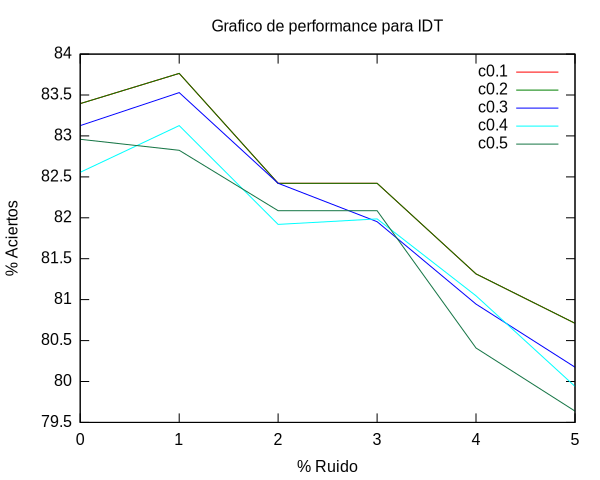
\includegraphics[scale=0.8]{../dats/idt.pdf}
\caption{Gráfico de aciertos de los distintos clasificadores \textsf{IDT} con confianza variable sobre ruido variable.}\label{fig:idt}
\end{figure}

\begin{figure}[h]
\centering
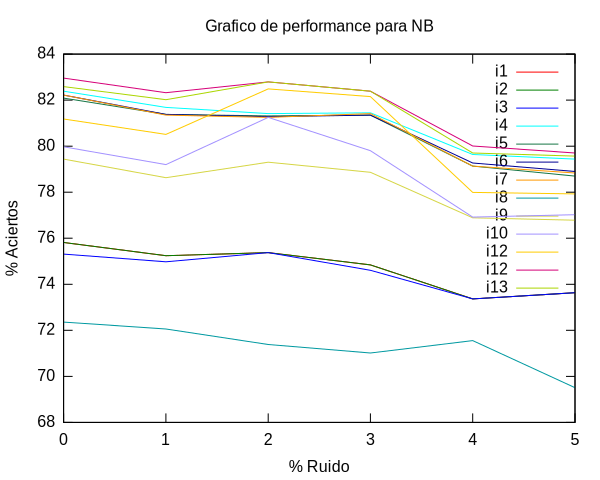
\includegraphics[scale=0.8]{../dats/nb.pdf}
\caption{Gráfico de aciertos de los distintos clasificadores \textsf{NB} con atributos variables sobre ruido variable.}\label{fig:nb}
\end{figure}

\begin{figure}[h]
\centering
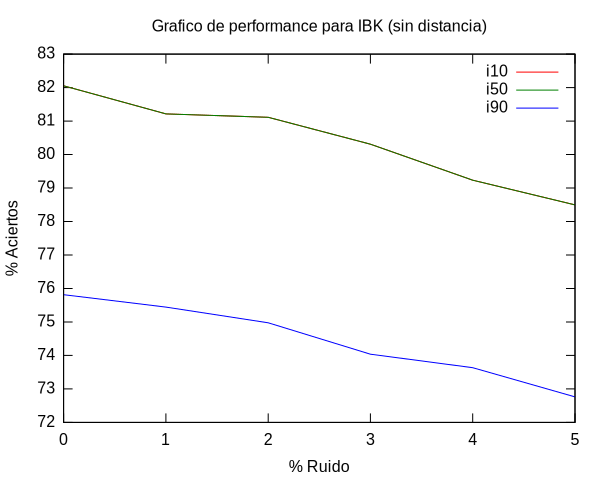
\includegraphics[scale=0.8]{../dats/ibk-no.pdf}
\caption{Gráfico de aciertos de los distintos clasificadores \textsf{IBk} con cantidad variable de instancias sobre ruido variable, sin ponderar las instancias.}\label{fig:ibk-no}
\end{figure}

\begin{figure}[h]
\centering
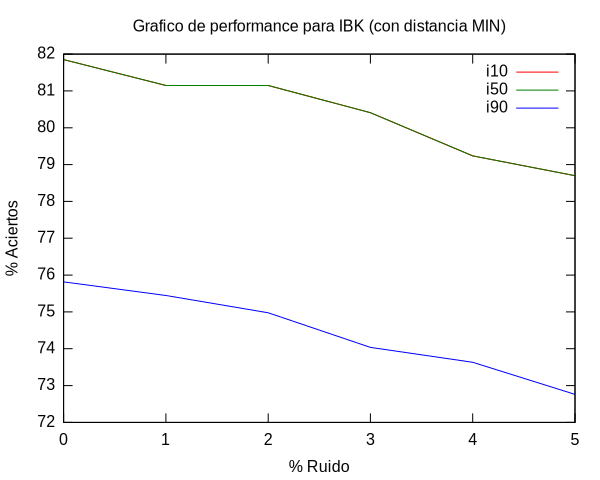
\includegraphics[scale=0.8]{../dats/ibk-min.pdf}
\caption{Gráfico de aciertos de los distintos clasificadores \textsf{IBk} con cantidad variable de instancias sobre ruido variable, con ponderación $1-d$.}\label{fig:ibk-min}
\end{figure}

\begin{figure}[h]
\centering
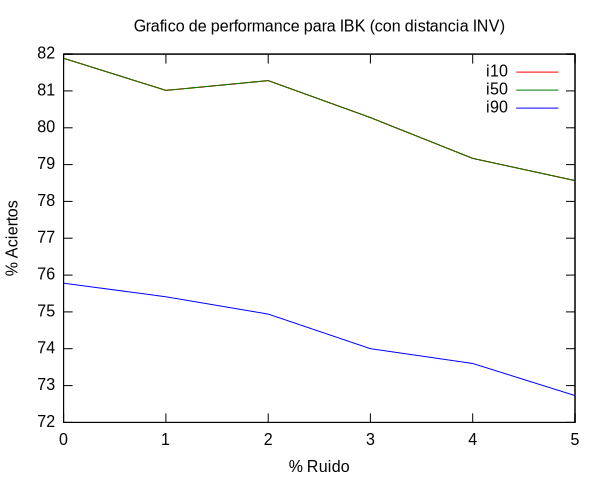
\includegraphics[scale=0.8]{../dats/ibk-inv.pdf}
\caption{Gráfico de aciertos de los distintos clasificadores \textsf{IBk} con cantidad variable de instancias sobre ruido variable, con ponderación $1/d$.}\label{fig:ibk-inv}
\end{figure}


Para los clasificadores \emph{basados en instancias} y de \emph{árboles de desición}, se utilizaron colores más oscuros para los clasificadores más específicos, según lo mencionado en la sección anterior. En el primer caso, el color oscuro se asignó a los clasificadores que utilizaban un vecindario más pequeño de instancias alrededor de la instancia a clasificar. En el segundo, se asignó a aquellos con mayor coeficiente de confianza, lo que daba lugar a un árbol con ramas más extensas que consideraban más atributos de la instancia. Para el gráfico de \textsf{naive bayes}, hubo un clasificador por cada tamaño de subconjunto de instancias a tomar, lo que no permitió utilizar un solo tono para los colores de las líneas. La designación i$x$ define cuantos atributos usando, siendo $x$ esta cantidad. \textsf{i1} es el clasificador menos específico, que toma en cuenta un único atributo.

En primer lugar tenemos un comportamiento generalizado para todas las técnicas en todas sus instancias: a mayor ruido peor performance, con el curioso evento donde a partir del 50\% de ruido aumenta el porcentaje de aciertos. Se entiende que pasado este 50\%, lo que se considaraba ruido pasa a ser cambiar la naturaleza de la clase, ya que en más de la mitad de los casos cambió la definición. En todos estos, la clase fue invertida, y ahora es el porcentaje restante de casos los que generan ruido para la nueva clasificación.

%Se debe tener en cuenta lo siguiente: al generar un $x\%$ de ruido no se modificaron aleatoriamente $x\%$ de instancias, pudiendo modificarse dos veces la misma instancia y dejándola en la misma clasificación; sino que se seguró que haya una cantidad equivalente a ese porcentaje con la clase cambiada. Esto significa que efectivamente el ruido 

Para los clasificadores utilizando \emph{árboles de desición} (fig \ref{fig:idt}) vemos que tuvieron siempre la mayor precisión aquellos que eran menos específicos, bajo la definición dada. Esto es, aquellos con árboles más chicos. En general, para estas técnicas, se busca reducir el tamaño del arbol (\emph{rule post-prunning}) para evitar que el clasificador esté sobreentrenado. Observamos que efectivamente esto ayuda a la precisión de la clasificación, en particular al crecer el ruido en los datos de entrenamiento.

Para los clasificadores \emph{probabilisticos}, vemos que con poco ruido los más problemáticos fueron aquellos con 1, 2, 3 y 7 atributos. Entre los mejores resultados se encuentran los que usan la mayoría de los atributos, y aquellos usando entre 4 y 6. El hecho que los mejores clasificadores estén muy distribuídos nos hace considerar que el test de $\chi^2$ no es suficiente para hacer una buena selección de atributos. De haber sido así se hubiera esperado que los mejores clasificadores hubieran estado agrupados hacia aquellos con menos atributos, pero con suficientes para tomar desiciones informadas. Si analizamos la \emph{performance} al incorporar atributos, entendemos que luego del cuarto atributo empezó a aparecer suficiente información, pero alrededor del séptimo aparecieron atributos conflictivos, lo cuál finalmente se compensó al tener información completa. Otro comportamiento observado fue que la diferencia en la precisión de los clasificadores disminuyó a medida que crecía el ruido.

En el caso de los clasificadores \emph{basados en instancias}, vemos que la función de distancia utilizada tuvo muy poco efecto en las capacidades de los clasificadores. Viendo los datos vemos que las diferencias para una misma cantidad de ruido no es mayor al 1\% de aciertos. En los tres casos tuvo el mejor resultado el clasificador utilizando un 10\% de las instancias cercanas al objetivo a clasificar. También sucedió que los clasificadores con 50 y 90\% de instancias estuvieron muy cerca en \emph{performance}. Otra observación es que la diferencia entre el más específico y los otros fue mucho más notoria a poco ruido y, en cambio, cerca del máximo de ruido hubo situaciones donde la cantidad de información de los menos específicos sirvió para compenzar el ruido y mejorar el porcentaje de aciertos. 

\section{Conclusiones}



\end{document}

